%!TEX root = ../DSGEnotes.tex
\chapter{DSGE模型求解方法简论}
\label{sec:solution-strat}


\section{简论的简论}
过去的三十多年来,宏观经济学研究经历了一场飞速变革。这场变革始于\cite{Kydland:1982cd}利用RBC模型研究美国经济。这种研究方法逐渐成为宏观经济学的标准范式之一\citep{An:2007cv, FernandezVillaverde:2010fq}。

随后RBC模型逐渐扩展到新凯恩斯主义模型。经典教材如\cite{Gali:2005gp,Woodford:2011ks}。然而新凯恩斯主义模型也远非完美无缺,随着新的问题逐渐被发现,学术界对模型做了进一步的修正和扩展,使模型对现实的拟合程度越来越高,如
\begin{itemize}
  \item 根据基准黏性价格假定所生成的一些重要经济变量的时间序列,与实际观察到的经济现实相比,出入较大——真实经济世界中的通货膨胀,产出,实际工资等时间序列数据都具有很高的持续性——为了使得模型与现实相贴近,模型设定中就需要引入看起来异常高的名义粘性。
  \item 因此产生了一系列对基准新凯恩斯模型的扩展,它们的基本思路是,加入\cite{Calvo:1983uq} 定价机制,从而可以在控制名义粘性不至于过高的情况下,有效提高模型生成的通货膨胀时间序列数据的持续性 \citep{Rabanal:2005ii}。
\end{itemize}

这样新凯恩斯主义分析框架得到了中央银行等政策制定者的青睐。不同中央银行开发了一系列自己的DSGE模型,如
\begin{itemize}
  \item 欧洲中央银行(ECB)的NAWM (New Ara-Wide Model)。

  在\cite{Fagan:2005hv}的Area-Wide Model (ARM)和\cite{Smets:2003ic}的基础上,\cite{Christoffel:2008vq} 开发了欧元区的NAWM,一个基于微观经济基础的开放经济模型,广泛应用于欧洲中央银行研究人员对经济系统的预测。
  \item 加拿大银行 (Bank of Canada)的ToTEM (Term-of-Trade Economic Model),见\cite{Murchison:2006wc}。
  \item 英格兰银行 (Bank of England)的BEQM (Bank of England Quarterly Model),见\cite{Harrison:2005tc}。
  \item 挪威银行 (Norges Bank)的NEMO (Norwegian Economy Model),见\cite{Brubakk:2006vu}。
  \item 智利中央银行(Central Bank of Chile)的MAS (Model of Analysis and Simulation), 见\cite{Medina:2007tz}。
  \item 瑞典中央银行 (Sveriges Riksbank)的RAMSES (Riksbanks Aggregated Model for Studies of the Economy in Sweden),见\cite{Adolfson:2007bv,Adolfson:2008cs}。
  \item 美联储的SIGMA。

  在\cite{Obstfeld:1995jp}的开放经济体模型基础上,\cite{Erceg:2006tf}简历的多国家开放经济模型。
  \item 国际货币基金组织(IMF)的GEM (Global Economic Model),见\cite{Bayoumi:2004vx}。
\end{itemize}

上述中央银行开发的经济预测模型,多得以于DSGE模型的长处,具有如下特征:
\begin{enumerate}
  \item 动态性。关注变量岁时间的变化路径,而不是某单独时间点上的情况。
  \item 整体性。致力于解释、预测整体经济运行,而非仅仅是局部市场。

  但这并不意味着DSGE模型可以重现整个经济系统的没一个重要部分,尤其是其中一些部门常常需要做必要的简化处理,如财政政策的制定部门(政府)、金融市场等。
  \item 重视部门均衡。根据经济学理论,在不同市场中,重视市场调节机制作用下的供应需求平衡。
  \item 模型中引入随机干扰。
\end{enumerate}

从广义的宏观经济学模型角度来看,DSGE模型可以分为两大类:RBC模型和新凯恩斯主义模型。RBC模型致力于研究在灵活价格环境下的经济周期波动,常表现为两部分的组合:一部分是随机内生经济增长模型作为内核,另一部分是外部真实技术冲击。\cite{Kydland:1982cd} 对RBC模型(进而DSGE模型)研究做出了开创性的贡献,进一步评述可见\cite{Cooley:1995tq}。

RBC关注实际经济变量,对货币问题未作深入讨论。而在现实经济世界中,货币的重要性越发得到重视。于是就有了新凯恩斯主义模型,大致说来,它对RBC模型做了两方面的扩展,一是一些内部机制的调整,二是外部冲击来源的选择。就前者而言,包括比如
\begin{enumerate}
  \item 将货币和货币发行机构(中央银行)引入到分析框架中来,
  \item 不再持有完全竞争假定,在一些部门的行为分析中假定不完全竞争,如:
  \begin{enumerate}
    \item 产品/服务市场,和/或劳动力市场是不完全竞争的,
    \item 允许私有部门的消费和投资决策在存在刚性的情况下展开:通过引入黏性价格、黏性工资的设定,将名义刚性引入模型设定中来。这意味着货币政策会对实际经济变量产生影响。
  \end{enumerate}
\end{enumerate}

如何构建一个DSGE模型,进而如何将其应用到宏观经济分析中去,仍需要我们在理论模型和计算求解两个维度上展开深入研究。就后者而言,很显然理论模型设定的细节不同,需要不同的求解方法。但总的说来,求解流程及方法大同小异:识别假设条件$\rightarrow$ 推出(一阶)均衡条件 $\rightarrow$ 构建结构方程组 $\rightarrow$ 形成随机差分方程系统(通常是非线性的) $\rightarrow$ \textbf{对非线性系统做近似线性化} $\rightarrow$ \textbf{求得近似解} $\rightarrow$ \textbf{(计算冲击响应方程或二阶矩以)检验近似解的有效度}。

本章主要对后半部分做简要介绍,大致包括DSGE模型的求解方法、参数估计、模型检验等。已有一系列文献对此作了综述,随着DSGE模型类型的不同,这些文献各有侧重,分别关注不同的求解方法,如
\begin{itemize}
  \item \cite{Canova:2009gc, Canova:2011vi, Balke:2012vl} 主要介绍常见的宏观计量经济学方法。
  \item \cite{An:2007cv, FernandezVillaverde:2010fq, DelNegro:2011wu, Herbst:2015wh}主要介绍贝叶斯估计法在DSGE模型中的应用。
  \item \cite{Gali:2005gp, Woodford:2011ks}主要关注DSGE模型的一种:新凯恩斯主义模型。
  \item \cite{Tovar:2009vb} 探讨DSGE模型在中央银行中的应用。
\end{itemize}

\section{pros and cons}
\subsection{cons}
目前学界基本达成共识,DSGE模型可作为宏观经济学研究的标准框架之一。但仍有局限,试从以下几个角度做简要介绍,分别为前提假定,求解方法,解的复杂性,以及利用解做决策的过程。

\textbf{前提假定}。一系列假定条件,如完美市场范式、市场效率、个体如家庭的理性期望等,引发争议。尤其是,过分简化、因而脱离实际的前提设定使得DSGE模型未能有效预测2008年的金融危机,使其广受质疑\citep{Buiter:2009ww}。作为回应,近年来的DSGE模型逐渐引入一些与现实更加贴近的假定,如个体行为的经验法则(rule-of-thumb),金融市场的摩擦,行为个体的异质性特征等。

\textbf{求解方法}。对本质上是高度非线性的经济系统而言,不恰当的近似线性化处理会导致损失许多重要信息,这些信息原本是宏观经济学研究的重要对象。\cite{Buiter:2009ww}甚至称之为``对宏观经济学模型的阉割''。

\textbf{解的复杂性,以及向公众解释政策含义的难度}。线性近似的最优条件和约束条件构成复杂而冗长的方程系统,在这系统中,第一,前向期望项变得难于辨认和解读,更难于向公众说明这一方程系统背后的经济学含义。第二,难于识别外生冲击如财政、货币政策的决策,是通过怎样的传导机制进入经济系统,并产生何种影响。第三,大多数情况下,难以直接求得系统的解析解,就需要借助计算机来测算近似的数值解,而采用何种数值算法更适合这一系统,数值近似解的精确程度如何,就成了又一个难题。这些都决定了模型系统及系统的解难以为公众们所理解,也因此难以在不同政策制定者之间形成共识。

\textbf{门槛高}。综上,DSGE模型的构建、求解、预测等一系列工作的展开,均要求研究者及政策制定者受过良好的宏观经济学训练,并有相当程度的建模能力、统计学知识和编程水平。

\subsection{pros}
尽管如此,采用DSGE模型作为宏观经济学研究分析框架的优势也很突出。

\textbf{微观基础}。传统宏观模型往往不对个体行为做深入设定。与之相比,DSGE模型在微观形为基础方面做了深入探索:行为个体基于理性预期的假定采取最优行动,决定要素价格和资源配置,进而影响公共部门的目标和约束条件。这样所生成的一系列局部最优条件,如家庭的劳动力供应决策、消费决策,企业的劳动力需求决策、产品定价决策等,为政策制定者提供重要参考依据。``优化''行为也意味着,个人和企业基于他们对未来期可能出现状况的预测,展开当前期的行为;从这种意义上来说,这种``理性预期''的行为模式便不同于``经验法则''。

\textbf{稳健性}。基于微观基础的DSGE模型使得缩减形式(reduced form)的参数与更深层次的结构形式(structural form)的参数之间,形成更紧密关联,使得模型参数较少可能随着政策的变动而发生变化——从此意义上说,DSGE模型有助于更稳健地回应卢卡斯批判\citep{Lucas:1976bm}\footnote{递归宏观经济学模型中的稳健控制论综述,可见\cite{Hansen:2004va}。简约式和结构式计量经济学方法论的争论,可见\cite{Jarrow:2004gy};一个更全面的综述可见\cite{Angrist:2008vkb}。}。

\textbf{模型研究与政策制定的契合度}。通过近似分散化经济体(decentralized economy)中典型个体的效用函数,DSGE模型产生与中心化经济(centralized economy)模型中的福利定律相一致的结果。从而,DSGE模型可以提供一套连贯的用于政策讨论与分析的工具,评估不同决策的效果,从而选取更好的决策付诸实施。在这一过程中,政策分析的展开与模型的设定条件是紧密相关的。

\textbf{工具包}。DSGE模型的吸引人之处不仅在于理论分析框架,更在于为宏观经济学的经验研究提供了一套可量化的政策分析和预测工具。伴随着理论建模的进展,也涌现出了很多新的经验工具和算法,致力于让模型分析的结果更贴近实际观察到的数据。随着二者相符程度的不断提升,DSGE模型的可靠性越来越得到政策制定机构如中央银行的认可\citep{An:2007cv},其预测效力不弱于VAR模型\cite{Edge:2010gp}。此外,模型估计方面的研究也有快速进展\citep{Schorfheide:2011tp, FernandezVillaverde:2016wy}。

总之,DSGE模型提供了一整套集成的政策分析框架。但仍需要指出两点。一,简化。经济模型始终是对现实世界的描述,这种描述是简化的,并不追求事无巨细的完整重现。那么研究人员基于DSGE模型给出的政策性建议都必须立足于常识,同时牢记简化了的模型并不覆盖纷繁复杂现实世界的每一个细节。二,主观性。一方面由于DSGE模型的复杂性,另一方面中央银行建立新的或改进已有的DSGE模型,目的往往是为自己的货币政策的有效性背书。在此过程中,主观性总是不可避免的。那么需要强调的是,基于DSGE模型的经济研究``不能代替专家意见'',政策制定者还需要考虑``坊间消息和模型之外的信息''\citep{Bernanke:2007vh}。

\section{工作流程}
设定前提假定条件$\rightarrow$求得系统解$\rightarrow$将模型生成的方针数据与实际观测到的数据向比较$\rightarrow$政策性建议,在分析无限时间周期的,由多个典型行为个体组成的DSGE模型时,常见的工作流程见下文,或如图\ref{fig:DSGE-work-flow}所示。
\begin{figure}[htbp]
   \caption{DSGE模型的工作流程}
  \centering
  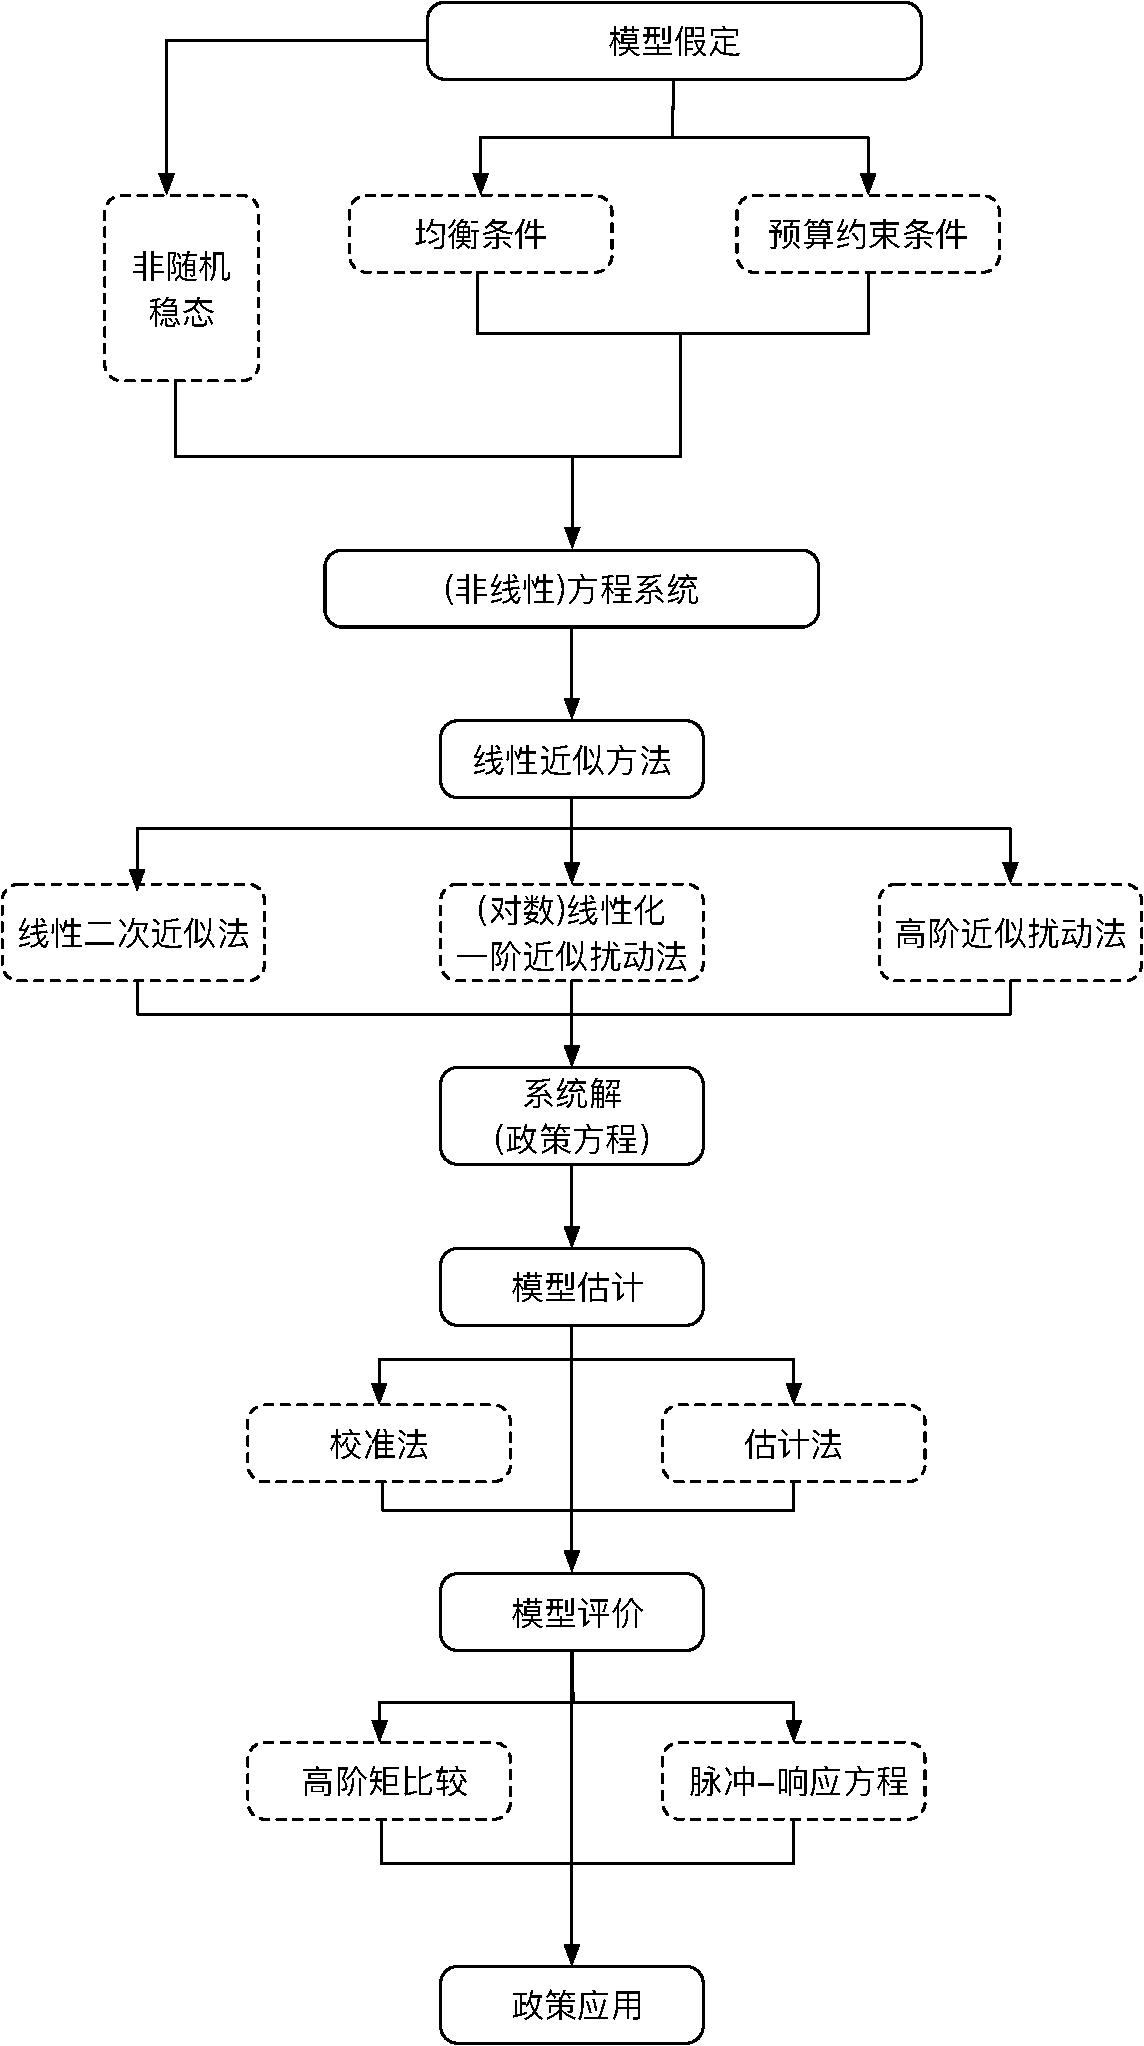
\includegraphics[height=13cm]{./Figures/20170701-DSGE-workflow}
  \label{fig:DSGE-work-flow}
%
%  \small{Source: PBOC.}
\end{figure}

\begin{enumerate}
  \item 构建经济模型(假设条件)。
  \item 求解一阶均衡条件。一阶均衡条件与预算约束条件等一道构成非线性随机差分方程系统。
  \item 由于该系统常常难以求得解析解,需要围绕这一个给定的点做数值近似。这一给定点,常常设定为模型的非随机稳定状态。
  \item 非随机稳定状态可由如下方法之一求得:
  \begin{enumerate}
    \item (对数)线性化近似,围绕稳态,得到一个状态——空间形式表述的线性差分系统,进而借助一些常见算法求得系统的近似数值解;
    \item 围绕非随机稳定状态,做二阶或更高阶的近似。
  \end{enumerate}
  \item 参数校准和/或估计。
  \item 针对外生随机冲击,计算方差、做方差分解,求得有关变量的脉冲——响应方程。
  \item 比较模型生成数据和史记观测到的数据以评价模型的解释力。
  \item 政策参考。
\end{enumerate}
下一节首先讨论模型设定。

\section{模型设定}
模型的前提假定应设定为与所研究的问题密切相关,并且必须指明模型中所讨论的问题是从定性还是定量的角度展开的。围绕所研究的问题,模型应该提供有所助益的回答,如:哪些冲击对经济体产生何种影响,它们的传导机制是怎样的,如何制定相关政策以应对这些冲击?

在一般均衡模型中,经济体中的每一个部门都是单独设定的,典型的部门如私人部门和公共部门:
\begin{enumerate}
  \item 私人部门包括如消费(家庭)部门和企业部门等。通常来说,消费者被简化为一个典型家庭,基于自身偏好,做关于消费和休闲的一生最优决策\citep{Christiano:2010wla}。企业在一定的生产条件限制下追求利润最大化。在为私人部门建模时,必须假定预期的形式,如理性预期或者经验法则等。
  \item 公共部门包括如财政政策和货币政策等。通常来说,政府是财政政策的制定者,大多数情况下财政政策的效果受到李嘉图等价(Ricardian equilvalence)的影响。中央银行设定货币政策。在为公共部门建模时,必须假定政策的执行方式,比如公共部门的政策制定是否依据某准则,是否受某种预算约束条件的限制,行为是否遵循某种利润最大化原则等。
  \item 在经济模型中,个体行动也要受到市场机制和制度性要素的考量,因此也徐作出设定,比如哪些市场是充分/非充分竞争的,决策者的政策制定是否需要遵循一些经验法则等。
  \item 外生随机冲击的识别和建模。
\end{enumerate}
上述模型设定都必须转换成适当的数学表达式,一方面使其能被纳入到模型分析框架中去,另一方面更重要的是,数学表达式的设定需要使模型有解。如,关于偏好和冲击的凹或凸的方程式,非庞兹骗局的约束条件等。

在模型设定后,下一步工作是要针对经济体中的家庭、企业、公共部门等,分别求得一阶最优条件和预算约束条件方程。这些方程常常包括当期和/或前向(后向)元素,又称非线性理性期望系统。通常来说,我们需要借助一定的数值近似方法,将非线性系统做近似线性化,进而求解,这一求解方法的讨论见下节。

\section{求解方法}
对于动态模型如新古典主义经济增长模型,最常见的解法是动态规划(Dynamic Programming),又称价值方程迭代,简要介绍见第\ref{sec:linear-quardratic-control-intro}章。这种方法的优势在于算法可靠度高,解的收敛特性好。但不足也较明显,如计算速度慢,存在维数灾难(curse of dimensionality, \cite{Bellman:1957tx})等\todo{curse of dimensionality,可由映射法得到一定程度上的缓解,做一个reference。}。

动态规划法的不足导致新算法的出现,典型如扰动法(perturbation methods)、投影法(projection methods)等。这些新方法在保持较好收敛特性的基础上,提供了更快的求解速度。扰动法在宏观经济学研究中的广泛应用,综述可见如\cite{Stokey1989,Ljungqvist:2004vz}。投影法的简要介绍见\cite{Aruoba:2006cz}。

本章内容重在对求解方法做简要介绍。大致说来,求解方法分为两步。第一步,近似线性化,将由均衡条件和约束条件构成的非线性方程系统转化为线性方程系统。不同方法背后核心思路基本一致,即将变量围绕其非随机稳定状态附近做线性近似。第二步常常被视为求解DSGE模型的核心,即根据近似线性系统的实际特征,采用相应的数值算法求解,作为原非线性系统的近似解\footnote{扰动法和投影法,从本质上来说都是局域算法。全局算法如车比雪夫多项式(Chebyshev-polynomial)、有限元(finite-elements)等的综述可见\cite{Judd:1998uy}。}。

\subsection{近似线性展开}
在\cite{King:1988bk, King:1988kf, King:2002ih}的开创性工作之后,(对数)线性近似法逐渐成为主要标准。以将变量沿着其非随机稳态做一节泰勒级数展开为例,假定$y=f(x)$,其中$x,y$分别是动态模型中的前定和非前定变量(predetermined and non-predetermined variables),$f$是个平滑的非线性函数\footnote{这里我们采用\cite{Klein:2000bc}的定义:$x_t$是前定变量,当且仅当它有外生的$1$期前向预测偏误,即$x_{t+1} - E_t X_{t+1} = C \varepsilon_{t+1}$是外生的。

根据这一定义,一个前定变量由它的滞后项和当期外生冲击所共同决定,如外生冲击变量。另一方面,不属于此情况的变量成为非前定变量,常常是前向变量。
}。

定义 $x_t$的确定性(非随机)稳定状态为$\bar{x}$,我们有$\bar{y} = \bar{x}$。

对$f$围绕$\bar{x}$做泰勒级数展开
\begin{equation}
  \label{sec:solution-talor-series-expansion-n}
  y \approx \sum_{n=0}^{\infty} \frac{f^{(n)}(\bar{x})}{n!} \left(x-\bar{x} \right)^{n},
\end{equation}
其中$f^{(n)}$表示$f$对$x$的第$n$次求导。

\subsubsection{(1阶)线性化近似}
根据\eqref{sec:solution-talor-series-expansion-n},1阶泰勒级数展开
\begin{equation}
  \label{sec:solution-talor-series-expansion-2-lin}
\begin{split}
    &y \approx f(\bar{x}) + f_x (\bar{x}) (x-\bar{x}), \\
    & \Rightarrow (y-\bar{y}) \approx f_x(\bar{x}) (x - \bar{x}), \\
    & \Rightarrow \frac{y-\bar{y}}{\bar{y}} \approx \frac{f_x (\bar{x}) \bar{x}}{\bar{y}} \frac{x - \bar{x}}{\bar{x}}, \\
    & \Rightarrow \tilde{y} \approx \underbrace{\frac{f_x (\bar{x}) \bar{x}}{\bar{y}}}_{\text{常系数}} \tilde{x},
\end{split}
\end{equation}
根据定义,$\tilde{y}_t$和$\tilde{x}_t$分别表示$y_t$和$x_t$相对于其确定性稳态$\bar{y}$和$\bar{x}$的偏离百分比。

\subsubsection{(1阶)对数线性化近似}
对模型做变型,$y=\exp(\ln y) = f(\exp (\ln x))$。

两侧取对数,$\ln y = \ln f(\exp (\ln x))$。

围绕$\ln \bar{x}$作1阶泰勒级数展开
\begin{equation}
  \begin{split}
    &\ln y \approx \ln f(\exp (\ln \bar{x})) + f_x (\bar{x}) \frac{d \exp(\ln x)}{d \bar{x}}  \left( \ln x - \ln \bar{x} \right), \\
    & \Rightarrow \ln y \approx \ln \bar{y} + f(\exp ( \ln \bar{x})) \left( \ln x - \ln \bar{x} \right), \\
    & \Rightarrow \ln \left(\frac{y}{\bar{y}}\right) \approx \underbrace{\frac{f_x (\bar{x}) \bar{x}}{\bar{y}}}_{\text{常系数}} \ln \left( \frac{x}{\bar{x}} \right),
  \end{split}
  \end{equation}
  其中$\ln \left(\frac{y}{\bar{y}}\right)$和$\ln \left( \frac{x}{\bar{x}} \right)$分别表示对数形式的偏离百分比。

一阶泰勒级数展开后的线性化近似和对数线性化近似,本质上相似。为了说明这一点,见下式
\begin{equation*}
  \tilde{x}_t = \frac{x_t - \bar{x}}{\bar{x}} = \frac{x_t}{\bar{x}} - 1 \approx \ln \left(\frac{x_t}{\bar{x}}\right) = \ln x_t - \ln \bar{x}.
\end{equation*}

此外\cite{Uhlig:1999vx}提出另一种类似对数线性化的方法,从而在特定情况下无需求导:对于常数$a$和接近$0$的$\tilde{x}_t$和$\tilde{y}_t$,
\begin{equation*}
  \begin{split}
    &\exp (x + ay) \approx 1 + x + ay, \\
    &\Rightarrow x y \approx 0, \\
    & \Rightarrow E_t \left( a \exp (x_{t+1}) \right) \approx E_t \left( a x_{t+1} \right).
  \end{split}
\end{equation*}

对数线性化方法的本质在于将变量$x_t$用$x \exp (\tilde{x}_t$来代替,此时$\tilde{x}_t = \ln (x_t/\bar{x})$表示它相对于稳态的对数偏差。利用此方法,可以将非线性方程近似为围绕稳态的线性方程。

\subsubsection{2阶近似}
根据\eqref{sec:solution-talor-series-expansion-n},以2阶展开为例
\begin{equation}
  \label{sec:solution-talor-series-expansion-2}
  y \approx \underbrace{f(\bar{x})}_{\text{0阶展开}} + \underbrace{f_{x}(\bar{x}) (x-\bar{x})}_{\text{1阶展开}} + \underbrace{\frac{1}{2} f_{xx}(\bar{x}) \left(x-\bar{x}\right)^2}_{\text{2阶展开}} + \underbrace{O^3}_{\text{误差项}},
\end{equation}
其中线性近似的误差项$O^3$是由忽略了3阶及以上阶数近似所造成的。

\eqref{sec:solution-talor-series-expansion-2}为代表的线性近似法具有如下特征:
\begin{enumerate}
  \item 在一阶泰勒级数展开中,$y$的条件期望值等于稳态下的$\bar{y}$,这意味着不确定性(以方差的二阶或更高阶矩等形式表现)在线性近似过程中不起作用。
  \item 在高阶泰勒级数展开中,$y$的条件期望值与方程$f$的曲率和变量$x$的方差有关。
  \item 如果研究的目的是求得冲击响应方程以及变量的二阶距,那么我们只分析模型的一阶属性即可,只需要对非线性系统做一阶泰勒级数展开。如,$var(y)$可以通过\eqref{sec:solution-talor-series-expansion-2}算出:$var(y) = E(y = Ey)^2 = f_x^2 var(x)$。
\end{enumerate}

在什么情况下做一阶展开,什么情况下需要做更高阶展开?
\begin{enumerate}
  \item 在很多情况下,对非线性系统做一阶线性近似即可。尽管有研究发现更高阶的近似会提供更精确的近似解,但精读提升的幅度有限。
  \item 然而的确存在一些情况,仅仅用一阶近似处理DSGE模型是不够的,尤其是当研究目标涉及到分析一些政策的福利效果时——这些福利政策往往不会对模型产生一阶影响。
\end{enumerate}
我们将在随后章节中进一步展开探讨这个问题\todo{加入一个reference。}。

对非线性方程系统做线性近似,生成以状态——空间形式表现的变型系统。这样,一方面可以更方便的展开后续经验研究,如模型估计,卡曼滤波,经济系统预测等。更为重要的是另一方面,搭配一些数值求解方法,可以求得系统的近似解。随后我们讨论如何在理性预期的情境下,运用数值算法求解变型系统。

\section{求解线性随机差分方程系统}
如前文所述,由各部门均衡条件和预算约束条件所组成的非线性系统,经由一定的(对数)线性化处理后变型为新的系统,又称线性随机方程差分系统,

新系统有一组含有理性期望条件的线性随机差分方程构成,可表述为如下状态——空间形式,
\begin{equation}
  \label{eq:solution-lin-stho-diff-eq}
  A_0 E_t Y_{t+1} = A_1 Y_t + B_0 \varepsilon_1,
\end{equation}
其中$A_0, A_1, B_0$是线性化系统的系数矩阵,$Y_t, \varepsilon_t$分别是内生变量和外生变量构成的向量。

在构建DSGE模型时,外生变量$\varepsilon_t$常取如下两个假定之一。假定$\varepsilon_t$是iid冲击向量,$E(\varepsilon_t) = 0, E(\varepsilon_t \varepsilon_t^{\top}) = \Sigma, E(\varepsilon_t \varepsilon_s^{\top}) = \Sigma \forall s \neq t$,或者假定$\varepsilon_t$是与iid外生冲击有关的$AR(1)$过程。

这样一个线性化方程构成的动态系统,描述了模型中变量的运动路径。通常来说系统中含有前向及后向要素\todo{Karl Whelan对 forward-looking和backward-looking的描述}。随着模型参数设定的不同,系统解存在三种情况:
\begin{itemize}
  \item 无解。系统没有稳定的理性预期解。
  \item 不确定(indeterminacy)。系统存在不止一个解的多重均衡。
  \item 确定的。有且只有一个解,又称稳定解。
\end{itemize}
如果前两种情况出现,意味着模型参数设定不当,需要重新调整,以使得系统存在稳定解。

已经有大量文献探讨理性期望系统\eqref{eq:solution-lin-stho-diff-eq}的求解方法。系统的解构成一个回应机制(feedback rule),将当期内生变量与模型内的状态变量联系起来。这方面的重要工作框架由\cite{Blanchard:1980gi}所奠定,随后经由许多人的努力,得到进一步深化和扩展,见第\ref{sec:rational-exp-chap}章。

如果DSGE模型致力于考察政策的福利效果,如期望效用等,则仅仅用一阶近似线性转换可能不够精确。此时需要对效用函数等其他函数做二阶近似,以确保二次项所含有的重要经济学信息不被忽略掉\citep{Kim:2003hf,SchmittGroh:2004da},见第\ref{sec:ptb}章。
